% Requires: \usepackage{graphicx,booktabs}

\section{Results and Analysis}

Figure~\ref{fig:combined-accuracy} summarizes our reproduced results across six
settings: full CIFAR-10/100, 10\% CIFAR-10/100, and 25\% CIFAR-10/100.  Compared
with the original paper trend in Figure~\ref{fig:paper-reported-accuracy}, our
absolute numbers are lower but the method ordering is similar: both
initialization methods improve over the default ViT initialization, and
Structured initialization is usually strongest.  On full CIFAR-10, accuracy
improves from 89.12\% for Default to 91.99\% for Mimetic and 92.47\% for
Structured.  On full CIFAR-100, the same ordering appears: 67.95\%, 72.67\%,
and 73.40\%.  This suggests that attention initialization is a useful way to
inject inductive bias without changing the ViT architecture.

\begin{figure}[H]
    \centering
    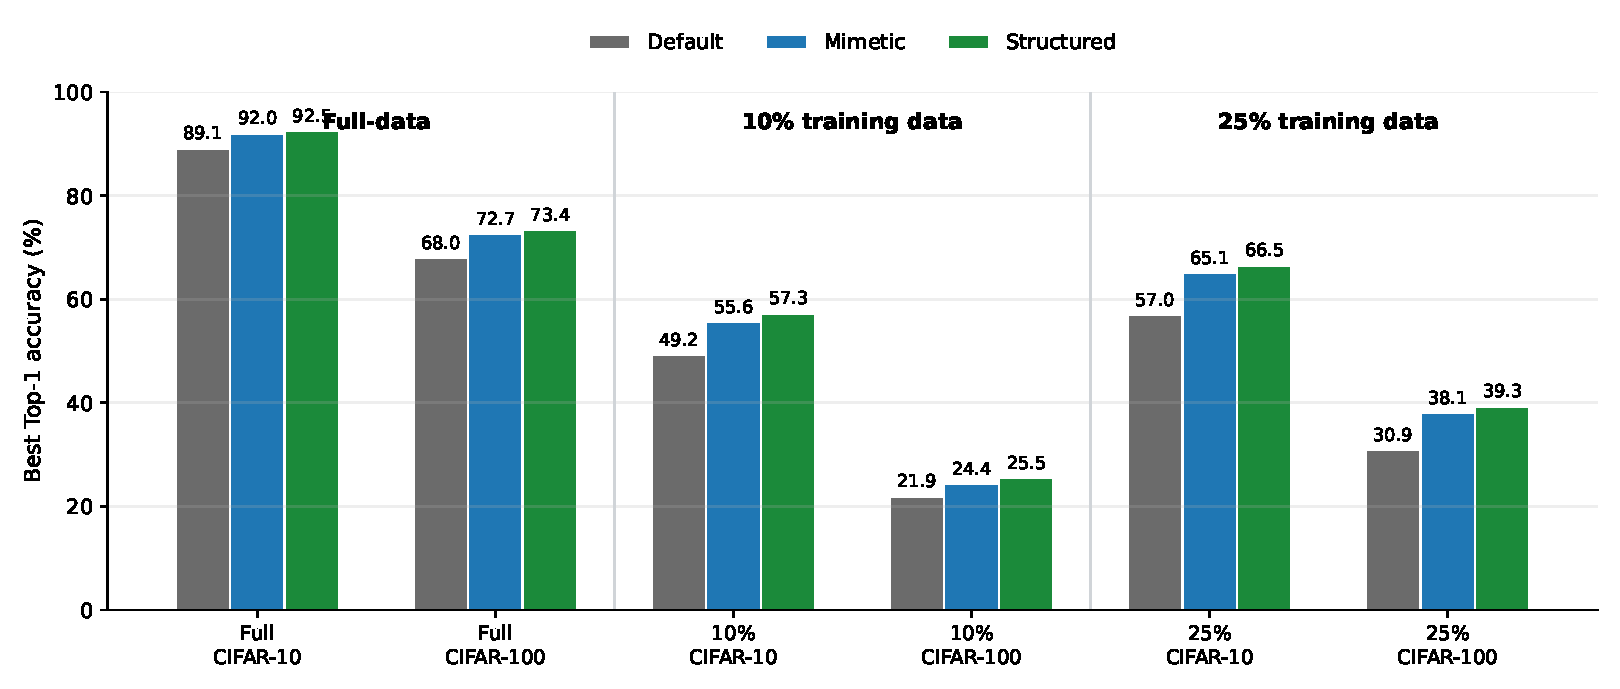
\includegraphics[width=\linewidth]{figures/fig_results_accuracy_combined.pdf}
    \caption{
    Best top-1 accuracy across full-data and low-data settings.  Structured
    initialization gives the best result in most settings, while Mimetic also
    consistently improves over the default baseline.
    }
    \label{fig:combined-accuracy}
\end{figure}

The advantage is especially visible in the low-data experiments.  With 10\% of
CIFAR-10, Mimetic improves over Default by 6.35 points, while Structured improves
by 8.06 points.  With 25\% of CIFAR-10, the gains become 8.17 and 9.58 points.
For CIFAR-100, Structured also improves over Default by 3.55 points at 10\% data
and 8.42 points at 25\% data.  These results support the small-data motivation:
when less supervision is available, a spatial attention prior helps the model
avoid learning locality completely from scratch.

Qualitatively, Mimetic helps by copying pretrained-like self-attention
statistics, while Structured is more explicit: it initializes query/key
attention to resemble local convolutional impulse filters.  The trained
attention maps in Figure~\ref{fig:attention-maps} provide a visual check:
Mimetic and Structured runs show clearer diagonal/local patterns than a purely
default initialization.  The L1/L6/L12 comparison also follows the original
paper visualization, where the impulse initialization produces strong local
diagonal attention.

\begin{figure}[H]
    \centering
    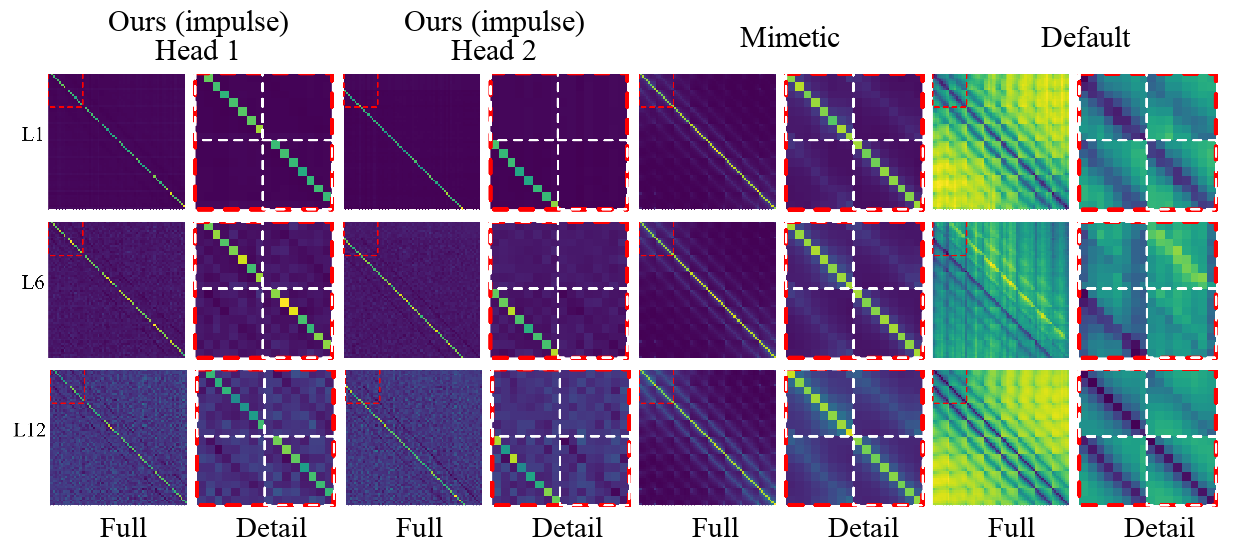
\includegraphics[width=\linewidth]{figures/fig_paper_attention_maps_l1_l6_l12.png}
    \vspace{0.2em}

    {\small (a) Original paper attention-map figure at L1, L6, and L12.}
    \vspace{0.45em}

    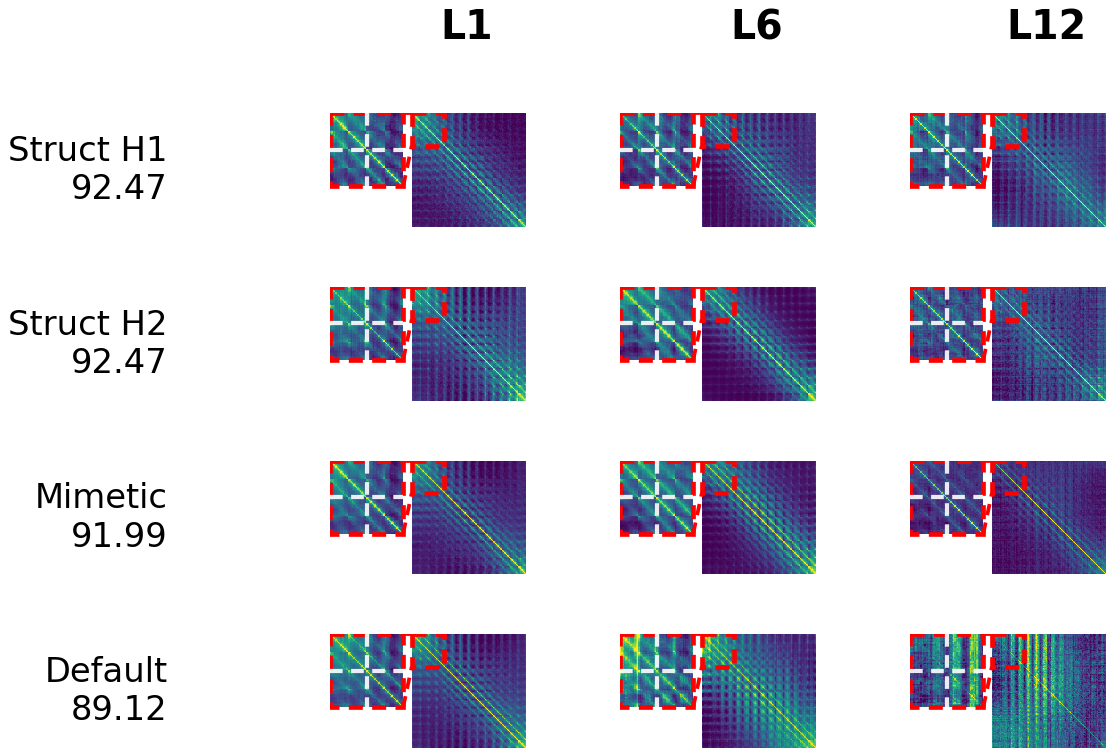
\includegraphics[width=0.86\linewidth]{figures/fig_attention_maps_cifar10.png}
    \vspace{0.2em}

    {\small (b) Our trained CIFAR-10 seed-0 checkpoint attention maps.}
    \caption{
    Attention-map comparison.  Both panels show patch-to-patch attention
    patterns at L1/L6/L12; brighter diagonal structures indicate stronger local
    patch attention.
    }
    \label{fig:attention-maps}
\end{figure}

Our absolute accuracies are still below the full results reported in the
original papers.  A likely reason is that our reproduction used a shorter
few-hundred-epoch training budget, fewer seed/hyperparameter sweeps, and an
independent reimplementation.  Therefore, the most important reproduced result
is the relative pattern rather than exact matching: Default $<$ Mimetic $<$
Structured in most full-data and low-data settings.

\begin{table}[H]
\centering
\small
\caption{CIFAR-10 seed stability under a common 250-epoch budget.}
\label{tab:seed-stability}
\begin{tabular}{lrrrr}
\toprule
Initialization & Seed 0 & Seed 1 & Seed 2 & Mean $\pm$ Std \\
\midrule
Default & 88.20 & 87.72 & 87.44 & 87.79 $\pm$ 0.38 \\
Mimetic & 91.32 & 91.03 & 90.42 & 90.92 $\pm$ 0.46 \\
Structured & 91.85 & 90.90 & 89.92 & 90.89 $\pm$ 0.97 \\
\bottomrule
\end{tabular}
\end{table}


The seed study adds an important caveat.  On CIFAR-10 at 250 epochs, Structured
is best for seed 0, but has higher variance across seeds (0.97 std) than Mimetic
(0.46 std) or Default (0.38 std).  This suggests that the stronger structured
locality prior can be more sensitive to the early training trajectory.  When the
prior aligns well with the data order and augmentation noise, it helps; when it
does not, the model may need more training to adapt from local attention toward
more task-specific attention patterns.

Figure~\ref{fig:training-curves} shows the corresponding training curves from
the exported logs.  Mimetic and Structured generally rise faster and end higher
than Default, so their advantage appears during optimization rather than only at
the final checkpoint.
